


% Header, overrides base

    % Make sure that the sphinx doc style knows who it inherits from.
    \def\sphinxdocclass{article}

    % Declare the document class
    \documentclass[letterpaper,10pt,english]{/home/tnaselar/anaconda/lib/python2.7/site-packages/sphinx/texinputs/sphinxhowto}

    % Imports
    \usepackage[utf8]{inputenc}
    \DeclareUnicodeCharacter{00A0}{\\nobreakspace}
    \usepackage[T1]{fontenc}
    \usepackage{babel}
    \usepackage{times}
    \usepackage{import}
    \usepackage[Bjarne]{/home/tnaselar/anaconda/lib/python2.7/site-packages/sphinx/texinputs/fncychap}
    \usepackage{longtable}
    \usepackage{/home/tnaselar/anaconda/lib/python2.7/site-packages/sphinx/texinputs/sphinx}
    \usepackage{multirow}

    \usepackage{amsmath}
    \usepackage{amssymb}
    \usepackage{ucs}
    \usepackage{enumerate}

    % Used to make the Input/Output rules follow around the contents.
    \usepackage{needspace}

    % Pygments requirements
    \usepackage{fancyvrb}
    \usepackage{color}
    % ansi colors additions
    \definecolor{darkgreen}{rgb}{.12,.54,.11}
    \definecolor{lightgray}{gray}{.95}
    \definecolor{brown}{rgb}{0.54,0.27,0.07}
    \definecolor{purple}{rgb}{0.5,0.0,0.5}
    \definecolor{darkgray}{gray}{0.25}
    \definecolor{lightred}{rgb}{1.0,0.39,0.28}
    \definecolor{lightgreen}{rgb}{0.48,0.99,0.0}
    \definecolor{lightblue}{rgb}{0.53,0.81,0.92}
    \definecolor{lightpurple}{rgb}{0.87,0.63,0.87}
    \definecolor{lightcyan}{rgb}{0.5,1.0,0.83}

    % Needed to box output/input
    \usepackage{tikz}
        \usetikzlibrary{calc,arrows,shadows}
    \usepackage[framemethod=tikz]{mdframed}

    \usepackage{alltt}

    % Used to load and display graphics
    \usepackage{graphicx}
    \graphicspath{ {figs/} }
    \usepackage[Export]{adjustbox} % To resize

    % used so that images for notebooks which have spaces in the name can still be included
    \usepackage{grffile}


    % For formatting output while also word wrapping.
    \usepackage{listings}
    \lstset{breaklines=true}
    \lstset{basicstyle=\small\ttfamily}
    \def\smaller{\fontsize{9.5pt}{9.5pt}\selectfont}

    %Pygments definitions
    
\makeatletter
\def\PY@reset{\let\PY@it=\relax \let\PY@bf=\relax%
    \let\PY@ul=\relax \let\PY@tc=\relax%
    \let\PY@bc=\relax \let\PY@ff=\relax}
\def\PY@tok#1{\csname PY@tok@#1\endcsname}
\def\PY@toks#1+{\ifx\relax#1\empty\else%
    \PY@tok{#1}\expandafter\PY@toks\fi}
\def\PY@do#1{\PY@bc{\PY@tc{\PY@ul{%
    \PY@it{\PY@bf{\PY@ff{#1}}}}}}}
\def\PY#1#2{\PY@reset\PY@toks#1+\relax+\PY@do{#2}}

\expandafter\def\csname PY@tok@gd\endcsname{\def\PY@tc##1{\textcolor[rgb]{0.63,0.00,0.00}{##1}}}
\expandafter\def\csname PY@tok@gu\endcsname{\let\PY@bf=\textbf\def\PY@tc##1{\textcolor[rgb]{0.50,0.00,0.50}{##1}}}
\expandafter\def\csname PY@tok@gt\endcsname{\def\PY@tc##1{\textcolor[rgb]{0.00,0.27,0.87}{##1}}}
\expandafter\def\csname PY@tok@gs\endcsname{\let\PY@bf=\textbf}
\expandafter\def\csname PY@tok@gr\endcsname{\def\PY@tc##1{\textcolor[rgb]{1.00,0.00,0.00}{##1}}}
\expandafter\def\csname PY@tok@cm\endcsname{\let\PY@it=\textit\def\PY@tc##1{\textcolor[rgb]{0.25,0.50,0.50}{##1}}}
\expandafter\def\csname PY@tok@vg\endcsname{\def\PY@tc##1{\textcolor[rgb]{0.10,0.09,0.49}{##1}}}
\expandafter\def\csname PY@tok@m\endcsname{\def\PY@tc##1{\textcolor[rgb]{0.40,0.40,0.40}{##1}}}
\expandafter\def\csname PY@tok@mh\endcsname{\def\PY@tc##1{\textcolor[rgb]{0.40,0.40,0.40}{##1}}}
\expandafter\def\csname PY@tok@go\endcsname{\def\PY@tc##1{\textcolor[rgb]{0.53,0.53,0.53}{##1}}}
\expandafter\def\csname PY@tok@ge\endcsname{\let\PY@it=\textit}
\expandafter\def\csname PY@tok@vc\endcsname{\def\PY@tc##1{\textcolor[rgb]{0.10,0.09,0.49}{##1}}}
\expandafter\def\csname PY@tok@il\endcsname{\def\PY@tc##1{\textcolor[rgb]{0.40,0.40,0.40}{##1}}}
\expandafter\def\csname PY@tok@cs\endcsname{\let\PY@it=\textit\def\PY@tc##1{\textcolor[rgb]{0.25,0.50,0.50}{##1}}}
\expandafter\def\csname PY@tok@cp\endcsname{\def\PY@tc##1{\textcolor[rgb]{0.74,0.48,0.00}{##1}}}
\expandafter\def\csname PY@tok@gi\endcsname{\def\PY@tc##1{\textcolor[rgb]{0.00,0.63,0.00}{##1}}}
\expandafter\def\csname PY@tok@gh\endcsname{\let\PY@bf=\textbf\def\PY@tc##1{\textcolor[rgb]{0.00,0.00,0.50}{##1}}}
\expandafter\def\csname PY@tok@ni\endcsname{\let\PY@bf=\textbf\def\PY@tc##1{\textcolor[rgb]{0.60,0.60,0.60}{##1}}}
\expandafter\def\csname PY@tok@nl\endcsname{\def\PY@tc##1{\textcolor[rgb]{0.63,0.63,0.00}{##1}}}
\expandafter\def\csname PY@tok@nn\endcsname{\let\PY@bf=\textbf\def\PY@tc##1{\textcolor[rgb]{0.00,0.00,1.00}{##1}}}
\expandafter\def\csname PY@tok@no\endcsname{\def\PY@tc##1{\textcolor[rgb]{0.53,0.00,0.00}{##1}}}
\expandafter\def\csname PY@tok@na\endcsname{\def\PY@tc##1{\textcolor[rgb]{0.49,0.56,0.16}{##1}}}
\expandafter\def\csname PY@tok@nb\endcsname{\def\PY@tc##1{\textcolor[rgb]{0.00,0.50,0.00}{##1}}}
\expandafter\def\csname PY@tok@nc\endcsname{\let\PY@bf=\textbf\def\PY@tc##1{\textcolor[rgb]{0.00,0.00,1.00}{##1}}}
\expandafter\def\csname PY@tok@nd\endcsname{\def\PY@tc##1{\textcolor[rgb]{0.67,0.13,1.00}{##1}}}
\expandafter\def\csname PY@tok@ne\endcsname{\let\PY@bf=\textbf\def\PY@tc##1{\textcolor[rgb]{0.82,0.25,0.23}{##1}}}
\expandafter\def\csname PY@tok@nf\endcsname{\def\PY@tc##1{\textcolor[rgb]{0.00,0.00,1.00}{##1}}}
\expandafter\def\csname PY@tok@si\endcsname{\let\PY@bf=\textbf\def\PY@tc##1{\textcolor[rgb]{0.73,0.40,0.53}{##1}}}
\expandafter\def\csname PY@tok@s2\endcsname{\def\PY@tc##1{\textcolor[rgb]{0.73,0.13,0.13}{##1}}}
\expandafter\def\csname PY@tok@vi\endcsname{\def\PY@tc##1{\textcolor[rgb]{0.10,0.09,0.49}{##1}}}
\expandafter\def\csname PY@tok@nt\endcsname{\let\PY@bf=\textbf\def\PY@tc##1{\textcolor[rgb]{0.00,0.50,0.00}{##1}}}
\expandafter\def\csname PY@tok@nv\endcsname{\def\PY@tc##1{\textcolor[rgb]{0.10,0.09,0.49}{##1}}}
\expandafter\def\csname PY@tok@s1\endcsname{\def\PY@tc##1{\textcolor[rgb]{0.73,0.13,0.13}{##1}}}
\expandafter\def\csname PY@tok@sh\endcsname{\def\PY@tc##1{\textcolor[rgb]{0.73,0.13,0.13}{##1}}}
\expandafter\def\csname PY@tok@sc\endcsname{\def\PY@tc##1{\textcolor[rgb]{0.73,0.13,0.13}{##1}}}
\expandafter\def\csname PY@tok@sx\endcsname{\def\PY@tc##1{\textcolor[rgb]{0.00,0.50,0.00}{##1}}}
\expandafter\def\csname PY@tok@bp\endcsname{\def\PY@tc##1{\textcolor[rgb]{0.00,0.50,0.00}{##1}}}
\expandafter\def\csname PY@tok@c1\endcsname{\let\PY@it=\textit\def\PY@tc##1{\textcolor[rgb]{0.25,0.50,0.50}{##1}}}
\expandafter\def\csname PY@tok@kc\endcsname{\let\PY@bf=\textbf\def\PY@tc##1{\textcolor[rgb]{0.00,0.50,0.00}{##1}}}
\expandafter\def\csname PY@tok@c\endcsname{\let\PY@it=\textit\def\PY@tc##1{\textcolor[rgb]{0.25,0.50,0.50}{##1}}}
\expandafter\def\csname PY@tok@mf\endcsname{\def\PY@tc##1{\textcolor[rgb]{0.40,0.40,0.40}{##1}}}
\expandafter\def\csname PY@tok@err\endcsname{\def\PY@bc##1{\setlength{\fboxsep}{0pt}\fcolorbox[rgb]{1.00,0.00,0.00}{1,1,1}{\strut ##1}}}
\expandafter\def\csname PY@tok@kd\endcsname{\let\PY@bf=\textbf\def\PY@tc##1{\textcolor[rgb]{0.00,0.50,0.00}{##1}}}
\expandafter\def\csname PY@tok@ss\endcsname{\def\PY@tc##1{\textcolor[rgb]{0.10,0.09,0.49}{##1}}}
\expandafter\def\csname PY@tok@sr\endcsname{\def\PY@tc##1{\textcolor[rgb]{0.73,0.40,0.53}{##1}}}
\expandafter\def\csname PY@tok@mo\endcsname{\def\PY@tc##1{\textcolor[rgb]{0.40,0.40,0.40}{##1}}}
\expandafter\def\csname PY@tok@kn\endcsname{\let\PY@bf=\textbf\def\PY@tc##1{\textcolor[rgb]{0.00,0.50,0.00}{##1}}}
\expandafter\def\csname PY@tok@mi\endcsname{\def\PY@tc##1{\textcolor[rgb]{0.40,0.40,0.40}{##1}}}
\expandafter\def\csname PY@tok@gp\endcsname{\let\PY@bf=\textbf\def\PY@tc##1{\textcolor[rgb]{0.00,0.00,0.50}{##1}}}
\expandafter\def\csname PY@tok@o\endcsname{\def\PY@tc##1{\textcolor[rgb]{0.40,0.40,0.40}{##1}}}
\expandafter\def\csname PY@tok@kr\endcsname{\let\PY@bf=\textbf\def\PY@tc##1{\textcolor[rgb]{0.00,0.50,0.00}{##1}}}
\expandafter\def\csname PY@tok@s\endcsname{\def\PY@tc##1{\textcolor[rgb]{0.73,0.13,0.13}{##1}}}
\expandafter\def\csname PY@tok@kp\endcsname{\def\PY@tc##1{\textcolor[rgb]{0.00,0.50,0.00}{##1}}}
\expandafter\def\csname PY@tok@w\endcsname{\def\PY@tc##1{\textcolor[rgb]{0.73,0.73,0.73}{##1}}}
\expandafter\def\csname PY@tok@kt\endcsname{\def\PY@tc##1{\textcolor[rgb]{0.69,0.00,0.25}{##1}}}
\expandafter\def\csname PY@tok@ow\endcsname{\let\PY@bf=\textbf\def\PY@tc##1{\textcolor[rgb]{0.67,0.13,1.00}{##1}}}
\expandafter\def\csname PY@tok@sb\endcsname{\def\PY@tc##1{\textcolor[rgb]{0.73,0.13,0.13}{##1}}}
\expandafter\def\csname PY@tok@k\endcsname{\let\PY@bf=\textbf\def\PY@tc##1{\textcolor[rgb]{0.00,0.50,0.00}{##1}}}
\expandafter\def\csname PY@tok@se\endcsname{\let\PY@bf=\textbf\def\PY@tc##1{\textcolor[rgb]{0.73,0.40,0.13}{##1}}}
\expandafter\def\csname PY@tok@sd\endcsname{\let\PY@it=\textit\def\PY@tc##1{\textcolor[rgb]{0.73,0.13,0.13}{##1}}}

\def\PYZbs{\char`\\}
\def\PYZus{\char`\_}
\def\PYZob{\char`\{}
\def\PYZcb{\char`\}}
\def\PYZca{\char`\^}
\def\PYZam{\char`\&}
\def\PYZlt{\char`\<}
\def\PYZgt{\char`\>}
\def\PYZsh{\char`\#}
\def\PYZpc{\char`\%}
\def\PYZdl{\char`\$}
\def\PYZhy{\char`\-}
\def\PYZsq{\char`\'}
\def\PYZdq{\char`\"}
\def\PYZti{\char`\~}
% for compatibility with earlier versions
\def\PYZat{@}
\def\PYZlb{[}
\def\PYZrb{]}
\makeatother


    %Set pygments styles if needed...
    
        \definecolor{nbframe-border}{rgb}{0.867,0.867,0.867}
        \definecolor{nbframe-bg}{rgb}{0.969,0.969,0.969}
        \definecolor{nbframe-in-prompt}{rgb}{0.0,0.0,0.502}
        \definecolor{nbframe-out-prompt}{rgb}{0.545,0.0,0.0}

        \newenvironment{ColorVerbatim}
        {\begin{mdframed}[%
            roundcorner=1.0pt, %
            backgroundcolor=nbframe-bg, %
            userdefinedwidth=1\linewidth, %
            leftmargin=0.1\linewidth, %
            innerleftmargin=0pt, %
            innerrightmargin=0pt, %
            linecolor=nbframe-border, %
            linewidth=1pt, %
            usetwoside=false, %
            everyline=true, %
            innerlinewidth=3pt, %
            innerlinecolor=nbframe-bg, %
            middlelinewidth=1pt, %
            middlelinecolor=nbframe-bg, %
            outerlinewidth=0.5pt, %
            outerlinecolor=nbframe-border, %
            needspace=0pt
        ]}
        {\end{mdframed}}
        
        \newenvironment{InvisibleVerbatim}
        {\begin{mdframed}[leftmargin=0.1\linewidth,innerleftmargin=3pt,innerrightmargin=3pt, userdefinedwidth=1\linewidth, linewidth=0pt, linecolor=white, usetwoside=false]}
        {\end{mdframed}}

        \renewenvironment{Verbatim}[1][\unskip]
        {\begin{alltt}\smaller}
        {\end{alltt}}
    

    % Help prevent overflowing lines due to urls and other hard-to-break 
    % entities.  This doesn't catch everything...
    \sloppy

    % Document level variables
    \title{test\_mix\_hog\_with\_fake\_data}
    \date{January 22, 2014}
    \release{}
    \author{Unknown Author}
    \renewcommand{\releasename}{}

    % TODO: Add option for the user to specify a logo for his/her export.
    \newcommand{\sphinxlogo}{}

    % Make the index page of the document.
    \makeindex

    % Import sphinx document type specifics.
     


% Body

    % Start of the document
    \begin{document}

        
            \maketitle
        

        


        
        \section{Represent an object map using a simple mixture-of-multinomials model}\subsubsection{create environment}

    % Make sure that atleast 4 lines are below the HR
    \needspace{4\baselineskip}

    
        \vspace{6pt}
        \makebox[0.1\linewidth]{\smaller\hfill\tt\color{nbframe-in-prompt}In\hspace{4pt}{[}68{]}:\hspace{4pt}}\\*
        \vspace{-2.65\baselineskip}
        \begin{ColorVerbatim}
            \vspace{-0.7\baselineskip}
            \begin{Verbatim}[commandchars=\\\{\}]
\PY{c}{\PYZsh{}create environment}
\PY{k+kn}{import} \PY{n+nn}{numpy} \PY{k+kn}{as} \PY{n+nn}{np}
\PY{k+kn}{from} \PY{n+nn}{PIL} \PY{k+kn}{import} \PY{n}{Image}
\PY{k+kn}{from} \PY{n+nn}{object\PYZus{}parsing.src.image\PYZus{}objects} \PY{k+kn}{import} \PY{n}{view\PYZus{}mask}
\PY{k+kn}{from} \PY{n+nn}{imagery\PYZus{}psychophysics.src.mixture\PYZus{}of\PYZus{}histograms} \PY{k+kn}{import} \PY{n}{mix\PYZus{}hog\PYZus{}image}\PY{p}{,} \PY{n}{plain\PYZus{}plot}
\PY{o}{\PYZpc{}}\PY{k}{pylab} \PY{n}{inline}
\end{Verbatim}

            
                \vspace{-0.2\baselineskip}
            
        \end{ColorVerbatim}
    

    

        % If the first block is an image, minipage the image.  Else
        % request a certain amount of space for the input text.
        \needspace{4\baselineskip}
        
        

            % Add document contents.
            
                \begin{InvisibleVerbatim}
                \vspace{-0.5\baselineskip}
\begin{alltt}Populating the interactive namespace from numpy and matplotlib
\end{alltt}

            \end{InvisibleVerbatim}
            
        
    
\subsubsection{model and simulation parameters}

    % Make sure that atleast 4 lines are below the HR
    \needspace{4\baselineskip}

    
        \vspace{6pt}
        \makebox[0.1\linewidth]{\smaller\hfill\tt\color{nbframe-in-prompt}In\hspace{4pt}{[}69{]}:\hspace{4pt}}\\*
        \vspace{-2.65\baselineskip}
        \begin{ColorVerbatim}
            \vspace{-0.7\baselineskip}
            \begin{Verbatim}[commandchars=\\\{\}]
\PY{c}{\PYZsh{}\PYZsh{}number of documents / probes}
\PY{n}{M} \PY{o}{=} \PY{l+m+mi}{500}

\PY{c}{\PYZsh{}\PYZsh{}number of pixels per document}
\PY{n}{P} \PY{o}{=} \PY{l+m+mi}{50}

\PY{c}{\PYZsh{}\PYZsh{}controls the uniformity of the initial guess at the prior distribution}
\PY{n}{UNIFORMITY} \PY{o}{=} \PY{l+m+mi}{1}

\PY{c}{\PYZsh{}\PYZsh{}controls how \PYZdq{}smooth\PYZdq{} the model parameter estimates are}
\PY{n}{SMOOTHING} \PY{o}{=} \PY{o}{.}\PY{l+m+mo}{0001}  \PY{c}{\PYZsh{}\PYZsh{} \PYZlt{}\PYZlt{} usually want number less than 1, it seems}
\end{Verbatim}

            
                \vspace{-0.2\baselineskip}
            
        \end{ColorVerbatim}
    
\subsubsection{grab an image / object map}

    % Make sure that atleast 4 lines are below the HR
    \needspace{4\baselineskip}

    
        \vspace{6pt}
        \makebox[0.1\linewidth]{\smaller\hfill\tt\color{nbframe-in-prompt}In\hspace{4pt}{[}70{]}:\hspace{4pt}}\\*
        \vspace{-2.65\baselineskip}
        \begin{ColorVerbatim}
            \vspace{-0.7\baselineskip}
            \begin{Verbatim}[commandchars=\\\{\}]
\PY{n}{cur\PYZus{}image} \PY{o}{=} \PY{l+m+mi}{3600}
\PY{n}{image\PYZus{}path} \PY{o}{=} \PY{l+s}{\PYZsq{}}\PY{l+s}{/musc.repo/Data/shared/my\PYZus{}labeled\PYZus{}images/pictures/}\PY{l+s+si}{\PYZpc{}0.6d}\PY{l+s}{.png}\PY{l+s}{\PYZsq{}}
\PY{n}{mask\PYZus{}path} \PY{o}{=} \PY{l+s}{\PYZsq{}}\PY{l+s}{/musc.repo/Data/shared/my\PYZus{}labeled\PYZus{}images/labeled\PYZus{}image\PYZus{}maps/}\PY{l+s+si}{\PYZpc{}0.6d}\PY{l+s}{.png}\PY{l+s}{\PYZsq{}}
\PY{n}{img} \PY{o}{=} \PY{n}{Image}\PY{o}{.}\PY{n}{open}\PY{p}{(}\PY{n}{image\PYZus{}path} \PY{o}{\PYZpc{}}\PY{p}{(}\PY{n}{cur\PYZus{}image}\PY{p}{)}\PY{p}{)}
\PY{n}{msk} \PY{o}{=} \PY{n}{Image}\PY{o}{.}\PY{n}{open}\PY{p}{(}\PY{n}{mask\PYZus{}path} \PY{o}{\PYZpc{}}\PY{p}{(}\PY{n}{cur\PYZus{}image}\PY{p}{)}\PY{p}{)}
\PY{n}{msk}\PY{o}{=}\PY{n}{msk}\PY{o}{.}\PY{n}{resize}\PY{p}{(}\PY{n}{size}\PY{o}{=}\PY{p}{(}\PY{l+m+mi}{64}\PY{p}{,}\PY{l+m+mi}{64}\PY{p}{)}\PY{p}{)}
\PY{n}{figure}\PY{p}{(}\PY{p}{)}
\PY{n}{plain\PYZus{}plot}\PY{p}{(}\PY{n}{gca}\PY{p}{(}\PY{p}{)}\PY{p}{)}
\PY{n}{title}\PY{p}{(}\PY{l+s}{\PYZsq{}}\PY{l+s}{original image}\PY{l+s}{\PYZsq{}}\PY{p}{)}
\PY{n}{imshow}\PY{p}{(}\PY{n}{img}\PY{p}{)}
\PY{n}{figure}\PY{p}{(}\PY{p}{)}
\PY{n}{plain\PYZus{}plot}\PY{p}{(}\PY{n}{gca}\PY{p}{(}\PY{p}{)}\PY{p}{)}
\PY{n}{title}\PY{p}{(}\PY{l+s}{\PYZsq{}}\PY{l+s}{object mask downsampled to 32x32}\PY{l+s}{\PYZsq{}}\PY{p}{)}
\PY{n}{imshow}\PY{p}{(}\PY{n}{msk}\PY{p}{)}
\PY{c}{\PYZsh{}view\PYZus{}mask(msk)}
\PY{n}{mask\PYZus{}array} \PY{o}{=} \PY{n}{np}\PY{o}{.}\PY{n}{array}\PY{p}{(}\PY{n}{msk}\PY{p}{)}
\PY{n}{N} \PY{o}{=} \PY{n}{mask\PYZus{}array}\PY{o}{.}\PY{n}{shape}
\PY{n}{V} \PY{o}{=} \PY{n}{np}\PY{o}{.}\PY{n}{prod}\PY{p}{(}\PY{n}{N}\PY{p}{)}
\PY{k}{print} \PY{l+s}{\PYZsq{}}\PY{l+s}{vocabulary size: }\PY{l+s+si}{\PYZpc{}d}\PY{l+s}{\PYZsq{}} \PY{o}{\PYZpc{}}\PY{p}{(}\PY{n}{V}\PY{p}{)}
\end{Verbatim}

            
                \vspace{-0.2\baselineskip}
            
        \end{ColorVerbatim}
    

    

        % If the first block is an image, minipage the image.  Else
        % request a certain amount of space for the input text.
        \needspace{4\baselineskip}
        
        

            % Add document contents.
            
                \begin{InvisibleVerbatim}
                \vspace{-0.5\baselineskip}
\begin{alltt}vocabulary size: 4096
\end{alltt}

            \end{InvisibleVerbatim}
            
                \begin{InvisibleVerbatim}
                \vspace{-0.5\baselineskip}
    \begin{center}
    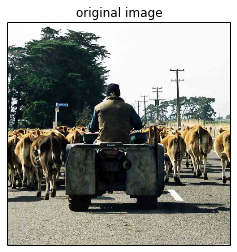
\includegraphics[max size={\textwidth}{\textheight}]{test_mix_hog_with_fake_data_files/test_mix_hog_with_fake_data_6_1.png}
    \par
    \end{center}
    
            \end{InvisibleVerbatim}
            
                \begin{InvisibleVerbatim}
                \vspace{-0.5\baselineskip}
    \begin{center}
    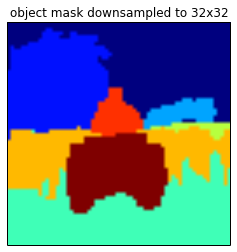
\includegraphics[max size={\textwidth}{\textheight}]{test_mix_hog_with_fake_data_files/test_mix_hog_with_fake_data_6_2.png}
    \par
    \end{center}
    
            \end{InvisibleVerbatim}
            
        
    
\subsubsection{represent the image mask as the parameters of a mixture-of-histograms
generative model}

    % Make sure that atleast 4 lines are below the HR
    \needspace{4\baselineskip}

    
        \vspace{6pt}
        \makebox[0.1\linewidth]{\smaller\hfill\tt\color{nbframe-in-prompt}In\hspace{4pt}{[}71{]}:\hspace{4pt}}\\*
        \vspace{-2.65\baselineskip}
        \begin{ColorVerbatim}
            \vspace{-0.7\baselineskip}
            \begin{Verbatim}[commandchars=\\\{\}]
\PY{c}{\PYZsh{}K = number of objects}
\PY{n}{K} \PY{o}{=} \PY{n+nb}{len}\PY{p}{(}\PY{n}{np}\PY{o}{.}\PY{n}{unique}\PY{p}{(}\PY{n}{mask\PYZus{}array}\PY{p}{)}\PY{p}{)}

\PY{c}{\PYZsh{}\PYZsh{}to create prior, count the number of pixels in each document}
\PY{n}{L} \PY{o}{=} \PY{p}{[}\PY{n+nb}{sum}\PY{p}{(}\PY{n+nb}{sum}\PY{p}{(}\PY{n}{mask\PYZus{}array}\PY{o}{==}\PY{n}{ii}\PY{p}{)}\PY{p}{)}\PY{o}{.}\PY{n}{astype}\PY{p}{(}\PY{l+s}{\PYZsq{}}\PY{l+s}{double}\PY{l+s}{\PYZsq{}}\PY{p}{)} \PY{k}{for} \PY{n}{ii} \PY{o+ow}{in} \PY{n}{np}\PY{o}{.}\PY{n}{arange}\PY{p}{(}\PY{n}{K}\PY{p}{)}\PY{o}{+}\PY{l+m+mi}{1}\PY{p}{]}
\PY{k}{print} \PY{l+s}{\PYZsq{}}\PY{l+s}{total number of pixels in each document:}\PY{l+s}{\PYZsq{}}
\PY{k}{print} \PY{n}{L}
\PY{k}{print}

\PY{n}{prior\PYZus{}dist} \PY{o}{=} \PY{n}{np}\PY{o}{.}\PY{n}{array}\PY{p}{(}\PY{n}{L}\PY{o}{/}\PY{n}{V}\PY{p}{)}\PY{o}{.}\PY{n}{reshape}\PY{p}{(}\PY{p}{(}\PY{l+m+mi}{1}\PY{p}{,}\PY{n}{K}\PY{p}{)}\PY{p}{)} \PY{c}{\PYZsh{}\PYZsh{}fraction of pixels in each object}
\PY{k}{print} \PY{l+s}{\PYZsq{}}\PY{l+s}{object prior:}\PY{l+s}{\PYZsq{}} 
\PY{k}{print} \PY{n}{prior\PYZus{}dist}

\PY{c}{\PYZsh{}\PYZsh{}to create the likelihood distributions, treat each object mask as the parameters of a multinomial}

\PY{c}{\PYZsh{}\PYZsh{}this just reformats the mask the way we want it to be}
\PY{k}{def} \PY{n+nf}{format\PYZus{}mask\PYZus{}as\PYZus{}lkhd}\PY{p}{(}\PY{p}{)}\PY{p}{:}
    \PY{k}{return} \PY{n}{np}\PY{o}{.}\PY{n}{hstack}\PY{p}{(}\PY{p}{[}\PY{n}{np}\PY{o}{.}\PY{n}{atleast\PYZus{}2d}\PY{p}{(}\PY{n}{np}\PY{o}{.}\PY{n}{array}\PY{p}{(}\PY{n}{mask\PYZus{}array}\PY{o}{==}\PY{n}{ii}\PY{p}{)}\PY{o}{.}\PY{n}{flatten}\PY{p}{(}\PY{p}{)}\PY{p}{)}\PY{o}{.}\PY{n}{T} \PY{k}{for} \PY{n}{ii} \PY{o+ow}{in} \PY{n}{np}\PY{o}{.}\PY{n}{arange}\PY{p}{(}\PY{n}{K}\PY{p}{)}\PY{o}{+}\PY{l+m+mi}{1}\PY{p}{]}\PY{p}{)}

\PY{c}{\PYZsh{}\PYZsh{}divide by total number of pixels to get a true probability instead of a count}
\PY{n}{lkhd\PYZus{}dist} \PY{o}{=} \PY{n}{format\PYZus{}mask\PYZus{}as\PYZus{}lkhd}\PY{p}{(}\PY{p}{)}\PY{o}{/}\PY{n}{L}

\PY{c}{\PYZsh{}\PYZsh{}If any pixel has 0 likelihood, set it to a very tiny number. this avoids lots of irritating bugs.}
\PY{n}{lkhd\PYZus{}dist} \PY{o}{=} \PY{n}{lkhd\PYZus{}dist} \PY{o}{+} \PY{n}{np}\PY{o}{.}\PY{n}{finfo}\PY{p}{(}\PY{n}{np}\PY{o}{.}\PY{n}{double}\PY{p}{)}\PY{o}{.}\PY{n}{tiny}

\PY{c}{\PYZsh{}\PYZsh{}re\PYZhy{}normalize to make sure each column still sums to 1}
\PY{n}{lkhd\PYZus{}dist} \PY{o}{=} \PY{n}{lkhd\PYZus{}dist}\PY{o}{/}\PY{n}{lkhd\PYZus{}dist}\PY{o}{.}\PY{n}{sum}\PY{p}{(}\PY{n}{axis}\PY{o}{=}\PY{l+m+mi}{0}\PY{p}{,} \PY{n}{keepdims}\PY{o}{=}\PY{n+nb+bp}{True}\PY{p}{)}
\end{Verbatim}

            
                \vspace{-0.2\baselineskip}
            
        \end{ColorVerbatim}
    

    

        % If the first block is an image, minipage the image.  Else
        % request a certain amount of space for the input text.
        \needspace{4\baselineskip}
        
        

            % Add document contents.
            
                \begin{InvisibleVerbatim}
                \vspace{-0.5\baselineskip}
\begin{alltt}total number of pixels in each document:
[1003.0, 712.0, 118.0, 1018.0, 47.0, 543.0, 134.0, 521.0]

object prior:
[[ 0.24487305  0.17382812  0.02880859  0.24853516  0.01147461
0.13256836
   0.03271484  0.12719727]]
\end{alltt}

            \end{InvisibleVerbatim}
            
        
    
\subsubsection{sample multiple ``probes'' from the ``true'' model}

    % Make sure that atleast 4 lines are below the HR
    \needspace{4\baselineskip}

    
        \vspace{6pt}
        \makebox[0.1\linewidth]{\smaller\hfill\tt\color{nbframe-in-prompt}In\hspace{4pt}{[}72{]}:\hspace{4pt}}\\*
        \vspace{-2.65\baselineskip}
        \begin{ColorVerbatim}
            \vspace{-0.7\baselineskip}
            \begin{Verbatim}[commandchars=\\\{\}]
\PY{n}{probes} \PY{o}{=} \PY{n}{np}\PY{o}{.}\PY{n}{zeros}\PY{p}{(}\PY{p}{(}\PY{n}{V}\PY{p}{,}\PY{n}{M}\PY{p}{)}\PY{p}{)}

\PY{c}{\PYZsh{}\PYZsh{}use prior to determine number of probes per object}
\PY{n}{probes\PYZus{}per\PYZus{}object} \PY{o}{=} \PY{n}{np}\PY{o}{.}\PY{n}{random}\PY{o}{.}\PY{n}{multinomial}\PY{p}{(}\PY{n}{M}\PY{p}{,} \PY{n}{np}\PY{o}{.}\PY{n}{squeeze}\PY{p}{(}\PY{n}{prior\PYZus{}dist}\PY{p}{)}\PY{p}{)}

\PY{c}{\PYZsh{}\PYZsh{}generate object patches}
\PY{n}{cnt} \PY{o}{=} \PY{l+m+mi}{0}
\PY{k}{for} \PY{n}{ii}\PY{p}{,}\PY{n}{nn} \PY{o+ow}{in} \PY{n+nb}{enumerate}\PY{p}{(}\PY{n}{probes\PYZus{}per\PYZus{}object}\PY{p}{)}\PY{p}{:}
    \PY{k}{for} \PY{n}{jj} \PY{o+ow}{in} \PY{n+nb}{range}\PY{p}{(}\PY{n}{nn}\PY{p}{)}\PY{p}{:}
        \PY{n}{dx} \PY{o}{=} \PY{n}{np}\PY{o}{.}\PY{n}{random}\PY{o}{.}\PY{n}{choice}\PY{p}{(}\PY{n}{np}\PY{o}{.}\PY{n}{arange}\PY{p}{(}\PY{n}{V}\PY{p}{)}\PY{p}{,} \PY{n}{size}\PY{o}{=}\PY{n}{P}\PY{p}{,} \PY{n}{replace}\PY{o}{=}\PY{n+nb+bp}{False}\PY{p}{,} \PY{n}{p}\PY{o}{=}\PY{n}{np}\PY{o}{.}\PY{n}{atleast\PYZus{}1d}\PY{p}{(}\PY{n}{lkhd\PYZus{}dist}\PY{p}{[}\PY{p}{:}\PY{p}{,}\PY{n}{ii}\PY{p}{]}\PY{p}{)}\PY{p}{)}
        \PY{n}{probes}\PY{p}{[}\PY{n}{dx}\PY{p}{,} \PY{n}{cnt}\PY{p}{]} \PY{o}{=} \PY{l+m+mi}{1}
        \PY{n}{cnt} \PY{o}{+}\PY{o}{=} \PY{l+m+mi}{1}

\PY{c}{\PYZsh{}\PYZsh{}check a few probes}
\PY{n}{figure}\PY{p}{(}\PY{p}{)}
\PY{n}{plain\PYZus{}plot}\PY{p}{(}\PY{n}{gca}\PY{p}{(}\PY{p}{)}\PY{p}{)}
\PY{n}{title}\PY{p}{(}\PY{l+s}{\PYZsq{}}\PY{l+s}{first probe}\PY{l+s}{\PYZsq{}}\PY{p}{)}
\PY{n}{imshow}\PY{p}{(}\PY{n}{probes}\PY{p}{[}\PY{p}{:}\PY{p}{,}\PY{l+m+mi}{0}\PY{p}{]}\PY{o}{.}\PY{n}{reshape}\PY{p}{(}\PY{n}{N}\PY{p}{)}\PY{p}{)}
\PY{n}{figure}\PY{p}{(}\PY{p}{)}
\PY{n}{plain\PYZus{}plot}\PY{p}{(}\PY{n}{gca}\PY{p}{(}\PY{p}{)}\PY{p}{)}
\PY{n}{title}\PY{p}{(}\PY{l+s}{\PYZsq{}}\PY{l+s}{last probe}\PY{l+s}{\PYZsq{}}\PY{p}{)}
\PY{n}{imshow}\PY{p}{(}\PY{n}{probes}\PY{p}{[}\PY{p}{:}\PY{p}{,}\PY{n}{M}\PY{o}{\PYZhy{}}\PY{l+m+mi}{1}\PY{p}{]}\PY{o}{.}\PY{n}{reshape}\PY{p}{(}\PY{n}{N}\PY{p}{)}\PY{p}{)}
\end{Verbatim}

            
                \vspace{-0.2\baselineskip}
            
        \end{ColorVerbatim}
    

    

        % If the first block is an image, minipage the image.  Else
        % request a certain amount of space for the input text.
        \needspace{4\baselineskip}
        
        

            % Add document contents.
            
                \makebox[0.1\linewidth]{\smaller\hfill\tt\color{nbframe-out-prompt}Out\hspace{4pt}{[}72{]}:\hspace{4pt}}\\*
                \vspace{-2.55\baselineskip}\begin{InvisibleVerbatim}
                \vspace{-0.5\baselineskip}
\begin{alltt}<matplotlib.image.AxesImage at 0x2861190>\end{alltt}

            \end{InvisibleVerbatim}
            
                \begin{InvisibleVerbatim}
                \vspace{-0.5\baselineskip}
    \begin{center}
    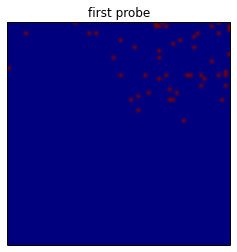
\includegraphics[max size={\textwidth}{\textheight}]{test_mix_hog_with_fake_data_files/test_mix_hog_with_fake_data_10_1.png}
    \par
    \end{center}
    
            \end{InvisibleVerbatim}
            
                \begin{InvisibleVerbatim}
                \vspace{-0.5\baselineskip}
    \begin{center}
    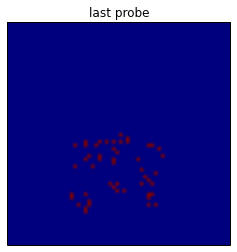
\includegraphics[max size={\textwidth}{\textheight}]{test_mix_hog_with_fake_data_files/test_mix_hog_with_fake_data_10_2.png}
    \par
    \end{center}
    
            \end{InvisibleVerbatim}
            
        
    
\subsubsection{initialize a naive model}

    % Make sure that atleast 4 lines are below the HR
    \needspace{4\baselineskip}

    
        \vspace{6pt}
        \makebox[0.1\linewidth]{\smaller\hfill\tt\color{nbframe-in-prompt}In\hspace{4pt}{[}73{]}:\hspace{4pt}}\\*
        \vspace{-2.65\baselineskip}
        \begin{ColorVerbatim}
            \vspace{-0.7\baselineskip}
            \begin{Verbatim}[commandchars=\\\{\}]
\PY{c}{\PYZsh{}\PYZsh{}prior and likelihood distributions are randomly sample from a dirichlet distribution}
\PY{n}{naive\PYZus{}prior\PYZus{}dist} \PY{o}{=} \PY{n}{np}\PY{o}{.}\PY{n}{random}\PY{o}{.}\PY{n}{dirichlet}\PY{p}{(}\PY{n}{UNIFORMITY}\PY{o}{*}\PY{n}{np}\PY{o}{.}\PY{n}{ones}\PY{p}{(}\PY{n}{K}\PY{p}{)}\PY{p}{)}\PY{o}{.}\PY{n}{reshape}\PY{p}{(}\PY{p}{(}\PY{l+m+mi}{1}\PY{p}{,}\PY{n}{K}\PY{p}{)}\PY{p}{)}
\PY{n}{naive\PYZus{}lkhd\PYZus{}dist} \PY{o}{=} \PY{n}{np}\PY{o}{.}\PY{n}{random}\PY{o}{.}\PY{n}{dirichlet}\PY{p}{(}\PY{n}{np}\PY{o}{.}\PY{n}{ones}\PY{p}{(}\PY{n}{V}\PY{p}{)}\PY{p}{,} \PY{n}{size}\PY{o}{=}\PY{n}{K}\PY{p}{)}\PY{o}{.}\PY{n}{T}

\PY{c}{\PYZsh{}\PYZsh{}instantiate a mixture of histograms model (image sub\PYZhy{}class)}
\PY{n}{mhi} \PY{o}{=} \PY{n}{mix\PYZus{}hog\PYZus{}image}\PY{p}{(}\PY{n}{naive\PYZus{}prior\PYZus{}dist}\PY{p}{,} \PY{n}{naive\PYZus{}lkhd\PYZus{}dist}\PY{p}{)}
\PY{k}{print} \PY{n}{mhi}\PY{o}{.}\PY{n}{prior\PYZus{}dist}
\end{Verbatim}

            
                \vspace{-0.2\baselineskip}
            
        \end{ColorVerbatim}
    

    

        % If the first block is an image, minipage the image.  Else
        % request a certain amount of space for the input text.
        \needspace{4\baselineskip}
        
        

            % Add document contents.
            
                \begin{InvisibleVerbatim}
                \vspace{-0.5\baselineskip}
\begin{alltt}[[ 0.00625544  0.07582994  0.16881811  0.17840073  0.12872255
0.10698929
   0.16031521  0.17466873]]
\end{alltt}

            \end{InvisibleVerbatim}
            
        
    
\subsubsection{\ldots{}and then restimate parameters}

    % Make sure that atleast 4 lines are below the HR
    \needspace{4\baselineskip}

    
        \vspace{6pt}
        \makebox[0.1\linewidth]{\smaller\hfill\tt\color{nbframe-in-prompt}In\hspace{4pt}{[}74{]}:\hspace{4pt}}\\*
        \vspace{-2.65\baselineskip}
        \begin{ColorVerbatim}
            \vspace{-0.7\baselineskip}
            \begin{Verbatim}[commandchars=\\\{\}]
\PY{c}{\PYZsh{}\PYZsh{}EM}
\PY{k}{print}\PY{p}{(}\PY{l+s}{\PYZsq{}}\PY{l+s}{the log\PYZhy{}likelihood of the data, given the current best estimate of the model parameters}\PY{l+s}{\PYZsq{}}\PY{p}{)}
\PY{n}{mhi}\PY{o}{.}\PY{n}{smoothing\PYZus{}param} \PY{o}{=} \PY{n}{SMOOTHING}
\PY{n}{mhi}\PY{o}{.}\PY{n}{run\PYZus{}em}\PY{p}{(}\PY{n}{probes}\PY{p}{)}
\end{Verbatim}

            
                \vspace{-0.2\baselineskip}
            
        \end{ColorVerbatim}
    

    

        % If the first block is an image, minipage the image.  Else
        % request a certain amount of space for the input text.
        \needspace{4\baselineskip}
        
        

            % Add document contents.
            
                \begin{InvisibleVerbatim}
                \vspace{-0.5\baselineskip}
\begin{alltt}the log-likelihood of the data, given the current best estimate of the
model parameters
===-217107.22397
===-189046.65340
===-184704.97577
===-183311.49647
===-181029.75831
===-178805.01911
===-178476.76878
===-178397.88723
===-178393.38244
===-178214.59221
===-178110.84241
===-177990.60885
===-177787.15706
===-177551.25957
===-177370.08183
===-177112.19299
===-177049.08367
===-177049.08367
\end{alltt}

            \end{InvisibleVerbatim}
            
        
    
\subsubsection{visualize the model parameters and the MAP estimate of the object that
each pixel belongs to}

    % Make sure that atleast 4 lines are below the HR
    \needspace{4\baselineskip}

    
        \vspace{6pt}
        \makebox[0.1\linewidth]{\smaller\hfill\tt\color{nbframe-in-prompt}In\hspace{4pt}{[}75{]}:\hspace{4pt}}\\*
        \vspace{-2.65\baselineskip}
        \begin{ColorVerbatim}
            \vspace{-0.7\baselineskip}
            \begin{Verbatim}[commandchars=\\\{\}]
\PY{k}{print} \PY{l+s}{\PYZsq{}}\PY{l+s}{(top) the likelihood distributions}\PY{l+s}{\PYZsq{}}
\PY{n}{mhi}\PY{o}{.}\PY{n}{view\PYZus{}lkhd\PYZus{}dist}\PY{p}{(}\PY{p}{)}
\PY{k}{print} \PY{l+s}{\PYZsq{}}\PY{l+s}{(middle) the prior distribution}\PY{l+s}{\PYZsq{}}
\PY{n}{mhi}\PY{o}{.}\PY{n}{view\PYZus{}prior}\PY{p}{(}\PY{p}{)}
\PY{k}{print} \PY{l+s}{\PYZsq{}}\PY{l+s}{(bottom) the best estimate of object membership for each pixel}\PY{l+s}{\PYZsq{}}
\PY{n}{mhi}\PY{o}{.}\PY{n}{view\PYZus{}MAP}\PY{p}{(}\PY{p}{)}
\end{Verbatim}

            
                \vspace{-0.2\baselineskip}
            
        \end{ColorVerbatim}
    

    

        % If the first block is an image, minipage the image.  Else
        % request a certain amount of space for the input text.
        \needspace{4\baselineskip}
        
        

            % Add document contents.
            
                \begin{InvisibleVerbatim}
                \vspace{-0.5\baselineskip}
\begin{alltt}(top) the likelihood distributions
(middle) the prior distribution
(bottom) the best estimate of object membership for each pixel
\end{alltt}

            \end{InvisibleVerbatim}
            
                \begin{InvisibleVerbatim}
                \vspace{-0.5\baselineskip}
    \begin{center}
    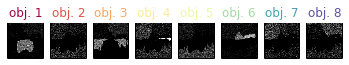
\includegraphics[max size={\textwidth}{\textheight}]{test_mix_hog_with_fake_data_files/test_mix_hog_with_fake_data_16_1.png}
    \par
    \end{center}
    
            \end{InvisibleVerbatim}
            
                \begin{InvisibleVerbatim}
                \vspace{-0.5\baselineskip}
    \begin{center}
    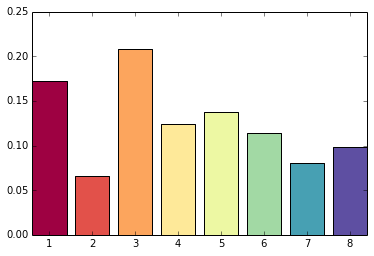
\includegraphics[max size={\textwidth}{\textheight}]{test_mix_hog_with_fake_data_files/test_mix_hog_with_fake_data_16_2.png}
    \par
    \end{center}
    
            \end{InvisibleVerbatim}
            
                \begin{InvisibleVerbatim}
                \vspace{-0.5\baselineskip}
    \begin{center}
    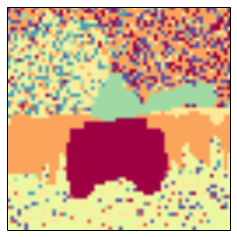
\includegraphics[max size={\textwidth}{\textheight}]{test_mix_hog_with_fake_data_files/test_mix_hog_with_fake_data_16_3.png}
    \par
    \end{center}
    
            \end{InvisibleVerbatim}
            
        
    
\subsubsection{now compare the MAP estimate to the original object mask}
        

        \renewcommand{\indexname}{Index}
        \printindex

    % End of document
    \end{document}


